The example below shows how to use the HyEQ solver to simulate a bouncing ball.

\begin{example}{bouncing ball with Lite HyEQ Solver}
\label{ex:bblite} Consider the hybrid system model for the bouncing ball with data given in Example~1.1.

For this example, we consider the ball to be bouncing on a floor at zero height. The constants for the bouncing ball system are $\gamma = 9.81$ and $\lambda=0.8$.
The following procedure is used to simulate this example in the Lite HyEQ Solver:
\begin{itemize}
\item Inside the MATLAB script {\tt run.m}, initial conditions, simulation horizons, a rule for jumps, ode solver options, and a step size coefficient are defined. The function {\tt HyEQsolver.m} is called in order to run the simulation, and a script for plotting solutions is included.
\item Then the MATLAB functions {\tt f.m, C.m, g.m, D.m} are edited according to the data given above.
\item Finally, the simulation is run by clicking the run button in {\tt run.m} or by calling {\tt run.m} in the MATLAB command window.
\end{itemize}

Example code for each of the MATLAB files {\tt run.m, f.m, C.m, g.m,} and {\tt D.m} is given below.\\

%\scriptsize
% This file was automatically created from the m-file 
% "m2tex.m" written by USL. 
% The fontencoding in this file is UTF-8. 
%  
% You will need to include the following two packages in 
% your LaTeX-Main-File. 
%  
% \usepackage{color} 
% \usepackage{fancyvrb} 
%  
% It is advised to use the following option for Inputenc 
% \usepackage[utf8]{inputenc} 
%  
  
% definition of matlab colors: 
\definecolor{mblue}{rgb}{0,0,1} 
\definecolor{mgreen}{rgb}{0.13333,0.5451,0.13333} 
\definecolor{mred}{rgb}{0.62745,0.12549,0.94118} 
\definecolor{mgrey}{rgb}{0.5,0.5,0.5} 
\definecolor{mdarkgrey}{rgb}{0.25,0.25,0.25} 
  
\DefineShortVerb[fontfamily=courier,fontseries=m]{\$} 
\DefineShortVerb[fontfamily=courier,fontseries=b]{\#} 
  
\noindent                                        
 \hspace*{-1.6em}{\scriptsize 1}$  $\color{mblue}$function$\color{black}$ run$\\
 \hspace*{-1.6em}{\scriptsize 2}$  $\color{mgreen}$% initial conditions$\color{black}$$\\
 \hspace*{-1.6em}{\scriptsize 3}$  x1_0 = 1;$\\
 \hspace*{-1.6em}{\scriptsize 4}$  x2_0 = 0;$\\
 \hspace*{-1.6em}{\scriptsize 5}$  x0 = [x1_0;x2_0];$\\
 \hspace*{-1.6em}{\scriptsize 6}$  $\color{mgreen}$% simulation horizon$\color{black}$$\\
 \hspace*{-1.6em}{\scriptsize 7}$  TSPAN=[0 $\color{mred}$10];$\color{black}$$\\
 \hspace*{-1.6em}{\scriptsize 8}$  JSPAN = [0 20];$\\
 \hspace*{-1.6em}{\scriptsize 9}$  $\color{mgreen}$% rule for jumps$\color{black}$$\\
 \hspace*{-2em}{\scriptsize 10}$  $\color{mgreen}$% rule = 1 -> priority for jumps$\color{black}$$\\
 \hspace*{-2em}{\scriptsize 11}$  $\color{mgreen}$% rule = 2 -> priority for flows$\color{black}$$\\
 \hspace*{-2em}{\scriptsize 12}$  rule = 1;$\\
 \hspace*{-2em}{\scriptsize 13}$  options = odeset($\color{mred}$'RelTol'$\color{black}$,1e-6,$\color{mred}$'MaxStep'$\color{black}$,.1);$\\
 \hspace*{-2em}{\scriptsize 14}$  $\color{mgreen}$% simulate$\color{black}$$\\
 \hspace*{-2em}{\scriptsize 15}$  [t,j,x] = HyEQsolver(@f,@g,@C,@D,x0,TSPAN,JSPAN,rule,options);$\\
 \hspace*{-2em}{\scriptsize 16}$  $\color{mgreen}$% plot solution$\color{black}$$\\
 \hspace*{-2em}{\scriptsize 17}$  figure(1) $\color{mgreen}$% position$\color{black}$$\\
 \hspace*{-2em}{\scriptsize 18}$  clf$\\
 \hspace*{-2em}{\scriptsize 19}$  subplot(2,1,1),plotflows(t,j,x(:,1))$\\
 \hspace*{-2em}{\scriptsize 20}$  grid $\color{mred}$on$\color{black}$$\\
 \hspace*{-2em}{\scriptsize 21}$  ylabel($\color{mred}$'x1'$\color{black}$)$\\
 \hspace*{-2em}{\scriptsize 22}$  subplot(2,1,2),plotjumps(t,j,x(:,1))$\\
 \hspace*{-2em}{\scriptsize 23}$  grid $\color{mred}$on$\color{black}$$\\
 \hspace*{-2em}{\scriptsize 24}$  ylabel($\color{mred}$'x1'$\color{black}$)$\\
 \hspace*{-2em}{\scriptsize 25}$  figure(2) $\color{mgreen}$% velocity$\color{black}$$\\
 \hspace*{-2em}{\scriptsize 26}$  clf$\\
 \hspace*{-2em}{\scriptsize 27}$  subplot(2,1,1),plotflows(t,j,x(:,2))$\\
 \hspace*{-2em}{\scriptsize 28}$  grid $\color{mred}$on$\color{black}$$\\
 \hspace*{-2em}{\scriptsize 29}$  ylabel($\color{mred}$'x2'$\color{black}$)$\\
 \hspace*{-2em}{\scriptsize 30}$  subplot(2,1,2),plotjumps(t,j,x(:,2))$\\
 \hspace*{-2em}{\scriptsize 31}$  grid $\color{mred}$on$\color{black}$$\\
 \hspace*{-2em}{\scriptsize 32}$  ylabel($\color{mred}$'x2'$\color{black}$)$\\
 \hspace*{-2em}{\scriptsize 33}$  $\color{mgreen}$% plot hybrid arc$\color{black}$$\\
 \hspace*{-2em}{\scriptsize 34}$  figure(3)$\\
 \hspace*{-2em}{\scriptsize 35}$  plotHybridArc(t,j,x)$\\
 \hspace*{-2em}{\scriptsize 36}$  xlabel($\color{mred}$'j'$\color{black}$)$\\
 \hspace*{-2em}{\scriptsize 37}$  ylabel($\color{mred}$'t'$\color{black}$)$\\
 \hspace*{-2em}{\scriptsize 38}$  zlabel($\color{mred}$'x1'$\color{black}$)$\\
 \hspace*{-2em}{\scriptsize 39}$  grid $\color{mred}$on$\color{black}$$\\
 \hspace*{-2em}{\scriptsize 40}$  view(37.5,30)$\\ 
  
\UndefineShortVerb{\$} 
\UndefineShortVerb{\#}\label{scr:run}
%\normalsize

%\scriptsize
% This file was automatically created from the m-file 
% "m2tex.m" written by USL. 
% The fontencoding in this file is UTF-8. 
%  
% You will need to include the following two packages in 
% your LaTeX-Main-File. 
%  
% \usepackage{color} 
% \usepackage{fancyvrb} 
%  
% It is advised to use the following option for Inputenc 
% \usepackage[utf8]{inputenc} 
%  
  
% definition of matlab colors: 
\definecolor{mblue}{rgb}{0,0,1} 
\definecolor{mgreen}{rgb}{0.13333,0.5451,0.13333} 
\definecolor{mred}{rgb}{0.62745,0.12549,0.94118} 
\definecolor{mgrey}{rgb}{0.5,0.5,0.5} 
\definecolor{mdarkgrey}{rgb}{0.25,0.25,0.25} 
  
\DefineShortVerb[fontfamily=courier,fontseries=m]{\$} 
\DefineShortVerb[fontfamily=courier,fontseries=b]{\#} 
  
\noindent                    
 \hspace*{-1.6em}{\scriptsize 1}$  $\color{mblue}$function$\color{black}$ xdot = f(x, u, gamma)$\\
 \hspace*{-1.6em}{\scriptsize 2}$  $\\
 \hspace*{-1.6em}{\scriptsize 3}$  $\color{mgreen}#%%%%%%%%%%%%%%%%%%%%%%%%%%%%%%%%%%%%%%%%%%%%%%%%%%%%%%%%%%%%%%%%%%%%%%%%%%%#\color{black}$$\\
 \hspace*{-1.6em}{\scriptsize 4}$  $\color{mgreen}$% Matlab Function  Author: Ricardo Sanfelice $\color{black}$$\\
 \hspace*{-1.6em}{\scriptsize 5}$  $\color{mgreen}$% (Revised by Giampiero Campa)$\color{black}$$\\
 \hspace*{-1.6em}{\scriptsize 6}$  $\color{mgreen}$% (Revised by Pablo Nanez)$\color{black}$$\\
 \hspace*{-1.6em}{\scriptsize 7}$  $\color{mgreen}$%$\color{black}$$\\
 \hspace*{-1.6em}{\scriptsize 8}$  $\color{mgreen}$% Project: Simulation of a hybrid system (Bouncing Ball)$\color{black}$$\\
 \hspace*{-1.6em}{\scriptsize 9}$  $\color{mgreen}$%$\color{black}$$\\
 \hspace*{-2em}{\scriptsize 10}$  $\color{mgreen}$% Name: f.m$\color{black}$$\\
 \hspace*{-2em}{\scriptsize 11}$  $\color{mgreen}$%$\color{black}$$\\
 \hspace*{-2em}{\scriptsize 12}$  $\color{mgreen}$% Description: Flow map$\color{black}$$\\
 \hspace*{-2em}{\scriptsize 13}$  $\color{mgreen}$%$\color{black}$$\\
 \hspace*{-2em}{\scriptsize 14}$  $\color{mgreen}$% Version: 1.0$\color{black}$$\\
 \hspace*{-2em}{\scriptsize 15}$  $\color{mgreen}$% Required files: - $\color{black}$$\\
 \hspace*{-2em}{\scriptsize 16}$  $\color{mgreen}#%%%%%%%%%%%%%%%%%%%%%%%%%%%%%%%%%%%%%%%%%%%%%%%%%%%%%%%%%%%%%%%%%%%%%%%%%%%#\color{black}$$\\
 \hspace*{-2em}{\scriptsize 17}$  $\\
 \hspace*{-2em}{\scriptsize 18}$  $\\
 \hspace*{-2em}{\scriptsize 19}$  $\color{mgreen}$% flow map: xdot=f(x,u);$\color{black}$$\\
 \hspace*{-2em}{\scriptsize 20}$  xdot = [x(2); gamma];$\\ 
  
\UndefineShortVerb{\$} 
\UndefineShortVerb{\#}\label{scr:f}
%\normalsize

%\scriptsize
% This file was automatically created from the m-file 
% "m2tex.m" written by USL. 
% The fontencoding in this file is UTF-8. 
%  
% You will need to include the following two packages in 
% your LaTeX-Main-File. 
%  
% \usepackage{color} 
% \usepackage{fancyvrb} 
%  
% It is advised to use the following option for Inputenc 
% \usepackage[utf8]{inputenc} 
%  
  
% definition of matlab colors: 
\definecolor{mblue}{rgb}{0,0,1} 
\definecolor{mgreen}{rgb}{0.13333,0.5451,0.13333} 
\definecolor{mred}{rgb}{0.62745,0.12549,0.94118} 
\definecolor{mgrey}{rgb}{0.5,0.5,0.5} 
\definecolor{mdarkgrey}{rgb}{0.25,0.25,0.25} 
  
\DefineShortVerb[fontfamily=courier,fontseries=m]{\$} 
\DefineShortVerb[fontfamily=courier,fontseries=b]{\#} 
  
\begin{Verbatim}[commandchars=\$\{\},numbers=left,numbersep=2pt] 

    $textcolor{mblue}{function} v  = C(x, u)  
     
    $textcolor{mgreen}{%%%%%%%%%%%%%%%%%%%%%%%%%%%%%%%%%%%%%%%%%%%%%%%%%%%%%%%%%%%%%%%%%%%%%%%%%%%} 
    $textcolor{mgreen} 
    $textcolor{mgreen} 
    $textcolor{mgreen} 
    $textcolor{mgreen} 
    $textcolor{mgreen}{% Version: 1.0} 
    $textcolor{mgreen}{% Required files: - } 
    $textcolor{mgreen}{%%%%%%%%%%%%%%%%%%%%%%%%%%%%%%%%%%%%%%%%%%%%%%%%%%%%%%%%%%%%%%%%%%%%%%%%%%%} 
     
    $textcolor{mgreen}{% state} 
    xi1 = x(1); 
    xi2 = x(2); 
     
    $textcolor{mgreen}{%input} 
    y2 = u(1); 
    v11 = u(2); 
    v12 = u(3); 
     
    $textcolor{mblue}{if} (xi1 >= y2)  $textcolor{mgreen}{% flow condition} 
        v = 1;  $textcolor{mgreen}{% report flow} 
    $textcolor{mblue}{else} 
        v = 0;   $textcolor{mgreen}{% do not report flow} 
    $textcolor{mblue}{end}  
\end{Verbatim}  
  
\UndefineShortVerb{\$} 
\UndefineShortVerb{\#} 
 \label{scr:C}
%\normalsize

%\scriptsize
% This file was automatically created from the m-file 
% "m2tex.m" written by USL. 
% The fontencoding in this file is UTF-8. 
%  
% You will need to include the following two packages in 
% your LaTeX-Main-File. 
%  
% \usepackage{color} 
% \usepackage{fancyvrb} 
%  
% It is advised to use the following option for Inputenc 
% \usepackage[utf8]{inputenc} 
%  
  
% definition of matlab colors: 
\definecolor{mblue}{rgb}{0,0,1} 
\definecolor{mgreen}{rgb}{0.13333,0.5451,0.13333} 
\definecolor{mred}{rgb}{0.62745,0.12549,0.94118} 
\definecolor{mgrey}{rgb}{0.5,0.5,0.5} 
\definecolor{mdarkgrey}{rgb}{0.25,0.25,0.25} 
  
\DefineShortVerb[fontfamily=courier,fontseries=m]{\$} 
\DefineShortVerb[fontfamily=courier,fontseries=b]{\#} 
  
\noindent                    
 \hspace*{-1.6em}{\scriptsize 1}$  $\color{mblue}$function$\color{black}$ xplus = g(x, u)$\\
 \hspace*{-1.6em}{\scriptsize 2}$  $\color{mgreen}$% state$\color{black}$$\\
 \hspace*{-1.6em}{\scriptsize 3}$  xi = z(statevect);$\\
 \hspace*{-1.6em}{\scriptsize 4}$  xi1 = xi(1);      $\color{mgreen}$%x-position$\color{black}$$\\
 \hspace*{-1.6em}{\scriptsize 5}$  xi2 = xi(2);      $\color{mgreen}$%y-position$\color{black}$$\\
 \hspace*{-1.6em}{\scriptsize 6}$  xi3 = xi(3);      $\color{mgreen}$%orientation angle$\color{black}$$\\
 \hspace*{-1.6em}{\scriptsize 7}$  q = xi(4);$\\
 \hspace*{-1.6em}{\scriptsize 8}$  $\color{mgreen}$% q = 1 --> going left$\color{black}$$\\
 \hspace*{-1.6em}{\scriptsize 9}$  $\color{mgreen}$% q = 2 --> going right$\color{black}$$\\
 \hspace*{-2em}{\scriptsize 10}$  xi1plus=xi1;$\\
 \hspace*{-2em}{\scriptsize 11}$  xi2plus=xi2;$\\
 \hspace*{-2em}{\scriptsize 12}$  xi3plus=xi3;$\\
 \hspace*{-2em}{\scriptsize 13}$  qplus=q;$\\
 \hspace*{-2em}{\scriptsize 14}$  $\color{mgreen}$% jump map$\color{black}$$\\
 \hspace*{-2em}{\scriptsize 15}$  $\color{mblue}$if$\color{black}$ ((xi1 >= 1) && (q == 2)) || ((xi1 <= -1) && (q == 1))$\\
 \hspace*{-2em}{\scriptsize 16}$     qplus = 3-q;$\\
 \hspace*{-2em}{\scriptsize 17}$  $\color{mblue}$else$\color{black}$$\\
 \hspace*{-2em}{\scriptsize 18}$      qplus = q;$\\
 \hspace*{-2em}{\scriptsize 19}$  $\color{mblue}$end$\color{black}$$\\
 \hspace*{-2em}{\scriptsize 20}$  xplus = [xi1plus;xi2plus;xi3plus;qplus];$\\ 
  
\UndefineShortVerb{\$} 
\UndefineShortVerb{\#}\label{scr:g}
%\normalsize

%\scriptsize
% This file was automatically created from the m-file 
% "m2tex.m" written by USL. 
% The fontencoding in this file is UTF-8. 
%  
% You will need to include the following two packages in 
% your LaTeX-Main-File. 
%  
% \usepackage{color} 
% \usepackage{fancyvrb} 
%  
% It is advised to use the following option for Inputenc 
% \usepackage[utf8]{inputenc} 
%  
  
% definition of matlab colors: 
\definecolor{mblue}{rgb}{0,0,1} 
\definecolor{mgreen}{rgb}{0.13333,0.5451,0.13333} 
\definecolor{mred}{rgb}{0.62745,0.12549,0.94118} 
\definecolor{mgrey}{rgb}{0.5,0.5,0.5} 
\definecolor{mdarkgrey}{rgb}{0.25,0.25,0.25} 
  
\DefineShortVerb[fontfamily=courier,fontseries=m]{\$} 
\DefineShortVerb[fontfamily=courier,fontseries=b]{\#} 
  
\noindent       
 \hspace*{-1.6em}{\scriptsize 1}$  $\color{mblue}$function$\color{black}$ v = D(x, u)$\\
 \hspace*{-1.6em}{\scriptsize 2}$  $\color{mgreen}$% jump set$\color{black}$$\\
 \hspace*{-1.6em}{\scriptsize 3}$  $\color{mblue}$if$\color{black}$ (x(1) <= u(1)) && (x(2) <= 0)  $\color{mgreen}$% jump condition$\color{black}$$\\
 \hspace*{-1.6em}{\scriptsize 4}$      v = 1;  $\color{mgreen}$% report jump$\color{black}$$\\
 \hspace*{-1.6em}{\scriptsize 5}$  $\color{mblue}$else$\color{black}$$\\
 \hspace*{-1.6em}{\scriptsize 6}$      v = 0;   $\color{mgreen}$% do not report jump$\color{black}$$\\
 \hspace*{-1.6em}{\scriptsize 7}$  $\color{mblue}$end$\color{black}$$\\ 
  
\UndefineShortVerb{\$} 
\UndefineShortVerb{\#}\label{scr:D}
%\normalsize

\begin{figure}[ht]
  \centering
  \psfrag{flows [t]}[c]{flows [$t$]}
  \psfrag{jumps [j]}[c]{jumps [$j$]}
  \psfrag{x1}[c]{$x_1$}
  \psfrag{x2}[c]{$x_2$}
\subfigure[Height]{
    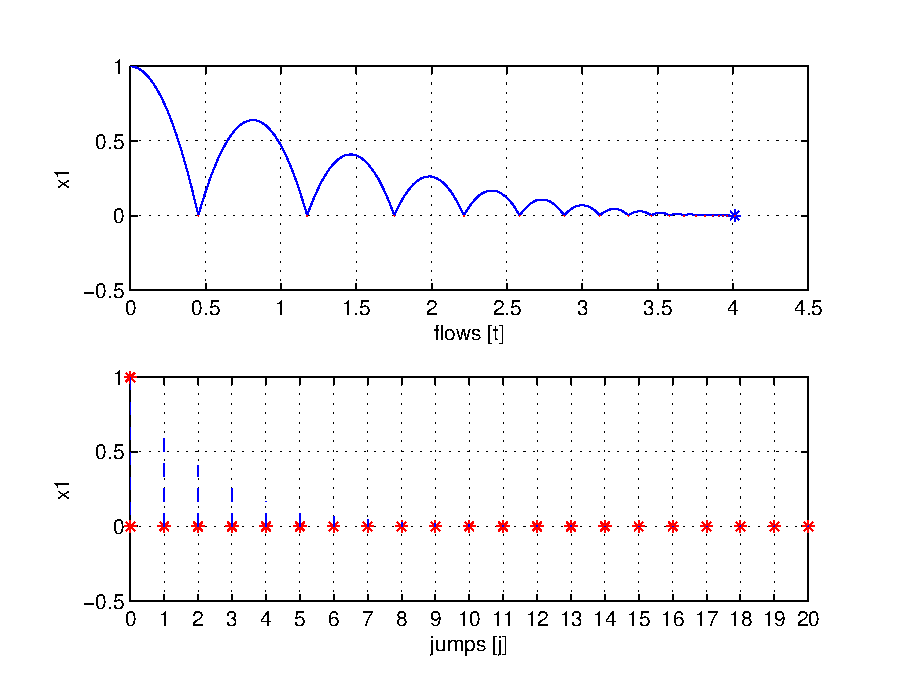
\includegraphics[width=.45\textwidth]{figures/Examples/FlowsAndJumps1lite.eps}
\label{fig:lite-1}}
\qquad
\subfigure[Velocity]{
    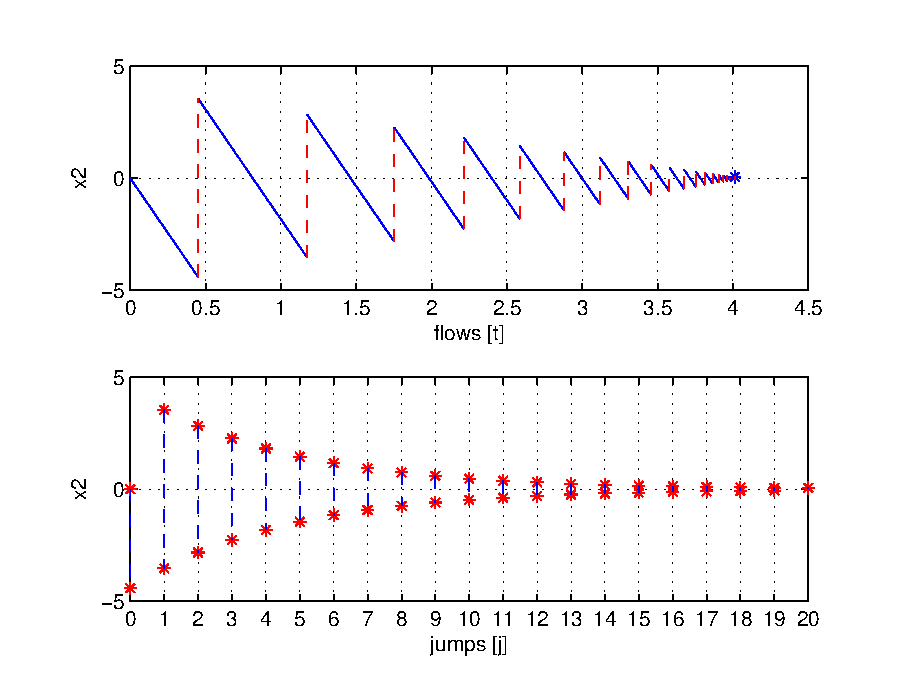
\includegraphics[width=.45\textwidth]{figures/Examples/FlowsAndJumps2lite.eps}
\label{fig:lite-2}}
\caption{Solution of Example \ref{ex:bblite}}
\end{figure}

\begin{figure}[ht]
  \begin{center}
  \psfrag{t}[c]{$t$}
  \psfrag{j}[c]{$j$}
  \psfrag{x1}[c]{$x_1$}
    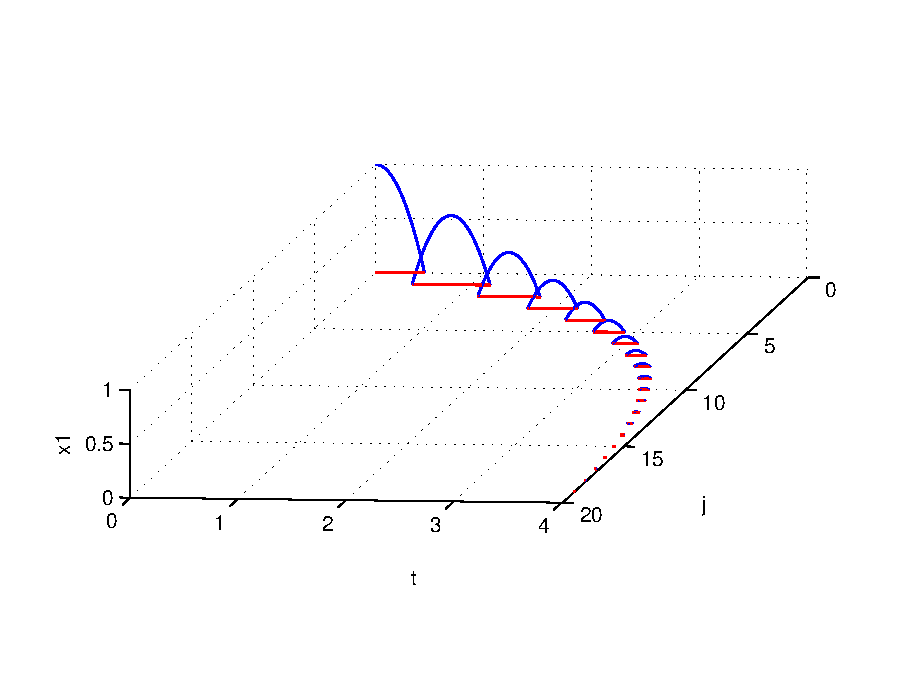
\includegraphics[width=.8\textwidth]{figures/Examples/HybridArclite.eps}
   \caption{Hybrid arc corresponding to a solution of Example~\ref{ex:bblite}: height}
\label{fig:lite-3}
  \end{center}
\end{figure}

A solution to the bouncing ball system from $x(0,0)=[1,0]^\top$ and with $TSPAN = [0 \hspace{2mm} 10], JSPAN = [0 \hspace{2mm} 20]$, $rule =1$, is depicted in Figure~\ref{fig:lite-1} (height) and Figure~\ref{fig:lite-2} (velocity).  Both the projection onto $t$ and $j$ are shown. Figure~\ref{fig:lite-3} depicts the corresponding hybrid arc for the position state.

For MATLAB files of this example, see Examples/Example\_\ref{ex:bblite}.

\end{example}
